\documentclass{article}

% Packages
\usepackage[utf8]{inputenc} % For modern characters
\usepackage{geometry}
\usepackage{microtype} % For sexy kerning
\usepackage{mathtools} % For math stuff
\usepackage{amssymb} % For math symbols
\usepackage{tabularx} % For making tables
\usepackage{listings} % For writing code
\usepackage{fancyhdr} % Use a header
\usepackage{pdfpages} % Include PDFs


% Other front matter
\lstset{language=R} % Set listing language to R
\newcommand{\code}[1]{\texttt{#1}}
\newcommand{\tab}{\hspace*{3em}} % Set tab spaces
\pagestyle{fancy}
\lhead{}
\chead{}
% Header for every page except the first two
\rhead{Ben Foster | Homework 2 | April 16, 2015} % Name, assignment, date
\setcounter{tocdepth}{2} % Set Table of Contents Depth
\setlength{\parindent}{0pt} % Disable automatic indentation


\begin{document}

% Title page, table of contents, and page number setting
{
	\title{Probability and Statistics for Engineers Homework Two \\ TMATH 390}
	\author{Ben Foster\thanks{
		Institute of Technology, University of Washington Tacoma} \\
		Instructor: Julia Eaton}
	\date{April 16, 2015}
	\maketitle
	\thispagestyle{empty} % Gets rid of the page number at the bottom
	\clearpage
	
	\pagenumbering{roman}
	\tableofcontents
	\clearpage
	\setcounter{page}{1}
	\pagenumbering{arabic}
}

%%% DONE
\section*{Problem 1} % Probably have to redo this because there is a different equation I might have to be using.
\addcontentsline{toc}{section}{First Problem}

	On her way to work, a friend of ours must pass through ten traffic signals. Suppose that in the 
	long run, she encounters a red light at 40\% of these signals and that whether any particular 
	signal is red is independent of whether any other one is red. (Note: what distribution could you 
	model this using? Is there an analogy of the red/green outcome with another variable that has a 
	binary outcome?) \\

	(a) On what proportion of days will our friend encounter at most two red lights? \\
	(b) On what proportion of days will our friend encounter at least five red lights? \\
	(c) On what proportion of days will our friend encounter between three and five (inclusive) red 	
	lights?

	\paragraph{Note:} We should model this using a binomial distribution. We could compare this 
	with the flip of a coin if the probability of getting heads in the long run was 40\% since each 
	individual coin flip result is also independent of one another and it is a binary answer. Also 
	note that we should not use the poisson approximation because we have a relatively large $\pi$ 
	and a relatively small $n$.

	\paragraph{Answer to a} Using R, we would determine the answer by typing in the command 
	\code{pbinom(2, 10, 0.4)} since we know that this is a binomial distribution. Here's how to do it 
	by hand using the equation $p(x) = \frac{n!}{(n-x)!x!}*p^{x} * (1-p)^{n-x}$ where $n=$ the 
	number of cases there are, $x=$ the number of successful encounters that day and $p=$ the 
	probability of getting a success:
	\begin{displaymath}
		p(x \le 2)  \sum_{x=0}^{2} \frac{10!}{(10-x)!x!}*0.4^{x} * (1-0.4)^{n-x}
	\end{displaymath}
	After doing the math required, we get an answer of: 0.167. %0.1672898

	\paragraph{Answer to b} Using R, we would use a similar command as the first problem: 
	\code{sum(dbinom(5:10, 10, 0.4))}. By hand we would also use a similar method, except this 
	time, we would use the equation:
	\begin{displaymath}
		p(x \ge 5)  \sum_{x=5}^{10} \frac{10!}{(10-x)!x!}*0.4^{x} * (1-0.4)^{n-x}
	\end{displaymath}
	After doing the math, we get an answer of 0.367. %0.3668967

	\paragraph{Answer to c} Using R, we would use a similar command as the first and second 
	problems: \code{sum(dbinom(3:5, 10, 0.4))}. By hand, we would also use a similar method, 
	except this time, we would use the equation:
	\begin{displaymath}
		p(3 \le x \le 5)  \sum_{x=3}^{5} \frac{10!}{(10-x)!x!}*0.4^{x} * (1-0.4)^{n-x}
	\end{displaymath}
	After doing the math, we get an answer of 0.666. %0.6664716

%%% DONE
\section*{Problem 2}
\addcontentsline{toc}{section}{Second Problem}

	Suppose that the number of drivers who travel between a particular origin and destination 
	during a designated time period has a Poisson distribution with parameter $\lambda = 8$. In the 
	long run, in what proportion of time periods will the number of drivers \\

	(a) Be at most 4? \\
	(b) Exceed 8? \\
	(c) Between 6 and 10 (inclusive)?

	\paragraph{Answer to a} To solve this in R, we would input the command: \code{ppois(4,8)}. By 
	hand, we would use the equation $p(x) = \frac{e^{-\lambda}\lambda^x}{x!}$ where $\lambda = 
	8$, the average number of drivers in this particular region and $x=$ the number of drivers and 
	then sum it all together:
	\begin{displaymath}
		p(x \le 4) = \sum_{x=0}^{4} \frac{e^{-8}8^x}{x!}
	\end{displaymath}
	Once you sum up all of the necessary equations, then you get an answer of: 0.0996 
	%0.0996324005

\iffalse
	\begin{displaymath}
		p(4) = \frac{e^{-8}8^4}{4!} = 0.0573 %0.0572522885
	\end{displaymath}
	\begin{displaymath}
		p(3) = \frac{e^{-8}8^3}{3!} = 0.0286 %0.0286261442
	\end{displaymath}
	\begin{displaymath}
		p(2) = \frac{e^{-8}8^2}{2!} = 0.0107 %0.0107348041
	\end{displaymath}
	\begin{displaymath}
		p(1) = \frac{e^{-8}8^1}{1!} = 0.00268 %0.002683701
	\end{displaymath}
	\begin{displaymath}
		p(0) = \frac{e^{-8}8^0}{0!} = 0.000335 %0.000335426279
	\end{displaymath}
	To get the actual answer, we need to sum together all of these.
	\begin{displaymath}
		p(4 \le x) = \sum_{x=0}^{4} \frac{e^{-8}8^x}{x!} = 0.0996 % 0.0996324005
	\end{displaymath}
\fi
	
	\paragraph{Answer to b} To solve this in R, we would use a similar command as part a: \code{1 
	- ppois(8, 8)}. By hand we would use the same equation except this time we are going to add 
	together the Poisson mass functions with $x \le 8$ and then subtract that answer from 1 in 
	order to get the proportion with $x > 8$: 
	\begin{displaymath}
		p(x \le 8) = \sum_{x=0}^{8} \frac{e^{-8}8^x}{x!} = 0.593 %0.5925473
	\end{displaymath}
	\begin{displaymath}
		p(x > 8) = 1 - p(x \le 8) = 0.407 %0.4074527
	\end{displaymath}
	After doing the math, we can see that the answer is 0.407.

\iffalse
	From the previous part:
	\begin{displaymath}
		p(4 \le x) = \sum_{x=0}^{4} \frac{e^{-8}8^x}{x!} = 0.0996 % 0.0996324005
	\end{displaymath}
	Therefore:
	\begin{displaymath}
		p(5) = \frac{e^{-8}8^5}{5!} = 0.0573 %0.0572522885
	\end{displaymath}
	\begin{displaymath}
		p(6) = \frac{e^{-8}8^6}{6!} = 0.0573 %0.0572522885
	\end{displaymath}
	\begin{displaymath}
		p(7) = \frac{e^{-8}8^7}{7!} = 0.0573 %0.0572522885
	\end{displaymath}
	\begin{displaymath}
		p(8) = \frac{e^{-8}8^8}{8!} = 0.0573 %0.0572522885
	\end{displaymath}
	Now we add the rest together and then subtract from one to get the actual answer.
\fi
	
	\paragraph{Answer to c} To solve this in R, we would use a similar command as part a and part b: \code{sum(dpois(6:10))}. By hand, we would use the same equation except this time we are going to just sum from $x=6$ to $x=10$. 
	\begin{displaymath}
		p(6 \le x \le 10) = \sum_{x=6}^{10} \frac{e^{-8}8^x}{x!}
	\end{displaymath}
	After doing the math, we get an answer of: 0.625. %0.6246497
	
%%% DONE
\clearpage
\section*{Problem 3}
\addcontentsline{toc}{section}{Third Problem}

	Let x denote the distance (m) that an animal moves from its birth site to the first territorial 
	vacancy it encounters. Suppose that for banner-tailed kangaroo rats, x has an exponential 
	distribution with parameter $\lambda = 0.01386$. \\

	(a) What proportion of distances are at most 80 m? \\
	(b) What proportion of distances are at least 60 m? \\
	(c) What is the median distance?

	\paragraph{Answer to a} To find the answer using R (which is the preferred method), you would 
	input the command: \code{sum(dexp(0:80, 0.01386))}. To do this by hand, we have to solve the 	exponential distribution equation:
	\begin{displaymath}
		p(x \le 80) = \sum_{x=0}^{80} 0.01386*e^{-0.01386*x}
	\end{displaymath}
	Which equals 0.679. %0.6792726
	
	\paragraph{Answer to b}  To find this answer using R, you would input a similar command: 
	\code{1 - sum(dexp(0:60, 0.01386))}. To do this by hand we would have to solve the equation:
	\begin{displaymath}
		p(x \ge 60) = \sum_{x=60}^{\infty} 0.01386*e^{-0.01386*x}
	\end{displaymath}
	After doing the math, you get 0.435. %0.435352
	
	\paragraph{Answer to c} To find this answer using R, you would input the command: 
	\code{qexp(0.5, 0.01386)}. To do this by hand you would have to solve the equation:
	\begin{displaymath}
		p(x) = \sum_{x=0}^{med} 0.01386*e^{-0.01386*x} = \frac{1}{2}
	\end{displaymath}
	Where $med$ is the median. After doing the math, you get an answer of 50.01. %50.01062

%%% DONE
\clearpage
\section*{Problem 4}
\addcontentsline{toc}{section}{Fourth Problem}

	Suppose that 10\% of all bits transmitted through a digital communication channel are 
	erroneously received and that whether any particular bit is erroneously received is independent 
	of whether any other bit is erroneously received. Consider sending a very large number of 
	messages, each consisting of 20 bits. \\

	(a) What proportion of these messages will have at most 2 erroneously received bits? \\
	(b) What proportion of these messages will have at least 5 erroneously received bits?

	\paragraph{Answer to a} This problem can be solved using the Binormal Distribution equation: 
	$p(x) = \frac{n!}{(n-x)!x!} * p^x * (1-p)^{n-x}$ where $n=$ the number of bits in each message, 
	$p=$ the probability of a bit is erroneously received and $x=$ the number of bits erroneously 
	received. To do this problem in R, we would input the command:
	\code{sum(dbinom(0:2,20,0.1))}. To do this by hand, we can input the variables to get the 
	equation:
	\begin{displaymath}
		p(x \le 2) = \sum_{x=0}^{2} \frac{20!}{(20-x)!x!} * 0.1^x * (1-0.1)^{20-x}
	\end{displaymath}
	From this, we get the answer: $p(x \le 2) = 0.677$. % 0.6769268
	
	\paragraph{answer to b} This problem is similar to the one above. Since we are finding the 
	proportion of messages that have \emph{at least 5} erroneous bits, then it would be easier to 
	just find the proportion of message with less than 5 erroneously received bits and then subtract 
	one. In R, all we would have to do is input the command: \code{sum(dbinom(5:20,20,0.1))}. To 
	do this by hand, we would use the equation:
	\begin{displaymath}
		p(x \ge 5) =1 - (\sum_{x=0}^{4} \frac{20!}{(20-x)!x!} * 0.1^x * (1-0.1)^{20-x})
	\end{displaymath}
	From this, we get the answer: $p(x \ge 5) = 0.0432$. %0.0431745

%%% DONE
\clearpage
\section*{Problem 5}
\addcontentsline{toc}{section}{Fifth Problem}

	Consider writing onto a computer disk and then sending it through a certifier that counts the 
	number of missing pulses. Suppose this number x has a Poisson distribution with parameter $
	\lambda = 0.2$. \\

	(a) What proportion of disks have exactly one missing pulse? \\
	(b) What proportion of disks have at least two missing pulses?

	\paragraph{Answer to a} To answer this problem in R, we would input the command: 
	\code{dpois(1, 0.2)}. By hand, we would use the equation
	\begin{displaymath}
		p(x) = \frac{e^{-\lambda}\lambda^x}{x!}
	\end{displaymath}
	Where $\lambda = 0.2$ and $x =$ the number of missing pulses. Filling in the variables of the equation, we end up with an answer of 0.164. %0.1637462
	
	\paragraph{Answer to b} To answer part b in R, we would take a somewhat similar approach, except this time, we would type in the command: \code{1 - sum(dpois(0:1, 0.2)}. We subtracted the value from 1 because we're looking for the proportion of \emph{at least} two missing pulses. By hand, we would just use the equation:
	\begin{displaymath}
		p(x \ge 2) = \sum_{x=0}^{1} \frac{e^{-\lambda}\lambda^x}{x!}
	\end{displaymath}
	From this, we get an answer of 0.0175. %0.0175231

%%% DONE
\section*{Problem 6}
\addcontentsline{toc}{section}{Sixth Problem}

	The bursting strength of wine bottles of a certain type is normally distributed with parameters $
	\mu = 250$ psi and $\sigma = 30$ psi. If these bottles are shipped 12 to a carton, in what 
	proportion of cartons will at least one of the bottles have a bursting strength exceeding 300 psi? 
	Hint: think of a bottle as a success, or "heads" $H$ if its bursting strength exceeds 300 psi.

	\paragraph{Answer} The answer to this question is a little complicated. Following the hint, we 
	would use a binormal distribution to show the proportion of cartons where at least one wine 
	bottle has burst. However, we need the probability that a wine bottle will burst in a carton. We 
	can find this by using the normal distribution and finding the proportion of bottles that burst 
	above 300 psi. Therefore, in R, we would input the command: \code{1 - dbinorm(0, 12, (1 - 
	pnorm(300, 250, 30)))}. \\
	
	To do this by hand, we would first have to use the equation $z = \frac{x-\mu}{\sigma}$ so that we can get the current normal distribution to a standard normal distribution and then we can just use our handout to get the value for when $x = 300$. From here, we use the number we got from the normal distribution, subtract it from 1, and then use that for the probability in the equation:
	\begin{displaymath}
		p(x \ge 1) = 1 - \frac{12!}{(12-0)!0!}*0.478^0*(1-0.478)^{12-0}
	\end{displaymath}
	Where we said $n = 12$, $x = 0$ and $p=$\code{(1 - pnorm(300, 250, 30))}. From this, we get an answer of 0.444. %0.4443633

%%%%%%%%%%%%%%%% Chapter Two Questions %%5%%%%%%%%%%%%%%%%

%%% DONE
\section*{Problem 7}
\addcontentsline{toc}{section}{Seventh Problem}

	Here are some data: 115.8, 115.2, 114.6, 115.9, 116.4. \\

	(a) Compute the mean of the deviations from the sample mean. (Note: the deviation of 
	observation $x_i$ from the mean $\bar{x}$ is $(x_i - \bar{x})$.) \\
	(b) Compute the sample standard deviation using the defining formula. \\
	(c) Compute it using the computational formula.
	
	Setting up tables like this will help: \\
	
	For parts (a) and (b):
	\begin{table}[!htb]
	\begin{tabular}{ | c | c | c | c | } \hline
		$i$ & $x_i$ & $x_i - \bar{x}$ & $(x_i - \bar{x})^2$ \\ \hline
		1 & 115.8 & & \\
		2 & 115.2 & & \\
		3 & 114.6 & & \\
		4 & 115.9 & & \\
		5 & 116.4 & & \\ \hline
		
		$n=5$ &
		$\sum_{i=1}^{5} x_i =$ &
		$\sum_{i=1}^{5}(x_i - \bar{x}) =$ &
		$ \sum_{i=1}^{5} (x_i - \bar{x})^2 =$ \\ 
		
		& $\bar{x} =$ & divide the above by $n$ for (a) & divide the above by $n-1$ for (b) \\ \hline
	\end{tabular}
	\end{table}
	
	For part (c):
	\begin{table}[!htb]
	\begin{tabular}{ | c | c | c | } \hline
		$i$ & $x_i$ & $(x_i)^2$ \\ \hline
		1 & 115.8 & \\
		2 & 115.2 & \\
		3 & 114.6 & \\
		4 & 115.9 & \\
		5 & 116.4 & \\ \hline
		& $\sum_{i=1}^{5} x_i =$ & $\sum_{i=1}^{5} (x_i)^2 =$ \\
		& $(\sum_{i=1}^{5} x_i)^2 =$ & \\ \hline
	\end{tabular}
	\end{table}
	Combine the two sums you computed using the "computation" formula to get (c).
	
	\paragraph{Answer to a and b} To find the answers to these two, we will fill in the first table 
	above. Also be sure to take the square root of $\frac{\sum_{i=1}^{5} (x_i - \bar{x})^2}{4}$ so that 
	we get the sample standard deviation:
	\begin{table}[!htb]
	\begin{tabular}{ | c | c | c | c | } \hline
		$i$ & $x_i$ & $|x_i - \bar{x}|$ & $(x_i - \bar{x})^2$ \\ \hline
		1 & 115.8 & 0.22 & 0.0484 \\
		2 & 115.2 & 0.38 & 0.1444 \\
		3 & 114.6 & 0.98 & 0.9604 \\
		4 & 115.9 & 0.32 & 0.1024 \\
		5 & 116.4 & 0.82 & 0.6724 \\ \hline
		
		$n=5$ &
		$\sum_{i=1}^{5} x_i =577.9$ &
		$\sum_{i=1}^{5}(x_i - \bar{x}) =2.72$ &
		$ \sum_{i=1}^{5} (x_i - \bar{x})^2 =1.928$ \\ 
		
		& $\bar{x} =115.58$ & (a) = 0.544 & (b) = 0.694 \\ \hline
	\end{tabular}
	\end{table}
	From the table we can see that the mean of the deviations from the sample mean is -0.72 and 
	the sample standard deviation is 1.13.
	
	\paragraph{Answer to c} To find the answer to c, we will fill in the second table above.
	\begin{table}[!htb]
	\begin{tabular}{ | c | c | c | } \hline
		$i$ & $x_i$ & $(x_i)^2$ \\ \hline
		1 & 115.8 & 13409.64 \\
		2 & 115.2 & 13271.04 \\
		3 & 114.6 & 13133.16 \\
		4 & 115.9 & 13432.81 \\
		5 & 116.4 & 13548.96 \\ \hline
		& $\sum_{i=1}^{5} x_i =577.9$ & $\sum_{i=1}^{5} (x_i)^2 =66795.61$ \\
		& $(\sum_{i=1}^{5} x_i)^2 =333968.41$ & \\ \hline
	\end{tabular}
	\end{table}
	
	The computational form for the standard deviation is:
	\begin{displaymath}
		s_x = \sqrt{\frac{1}{n-1}\left(\sum_{i=1}^{5}x_i^2-\frac{1}{n}\left(\sum_{i=1}^{5}x_i
		\right)^2\right)}
	\end{displaymath}
	\begin{displaymath}
		= \sqrt{\frac{1}{5-1}\left(66795.61 - \frac{333968.41}{5}\right)}
	\end{displaymath}
	\begin{displaymath}
		= 0.694
	\end{displaymath}

%%% DONE
\clearpage
\section*{Problem 8}
\addcontentsline{toc}{section}{Eighth Problem}

	Recall the uniform distribution, with the the density function
	\begin{displaymath}
		f(x) = \left\{
		\begin{array}{lr}
			\frac{1}{b-a}, & $if $ a < x < b \\
			0, & $otherwise$
		\end{array}
		\right.
	\end{displaymath}
	The corresponding density "curve" has constant height over the interval from $a$ to $b$. \\

	Compute the mean of the uniform distribution in terms of $a$ and $b$.

	\paragraph{Answer} Since the mean is the average of all the numbers and a uniform distribution 
	has the same height throughout the entire graph, then the mean distribution in terms of $a$ and 
	$b$ is: 
	\begin{displaymath}
		\frac{a+b}{2}
	\end{displaymath}
	Here's a more in-depth way of describing it:
	\begin{displaymath}
		E[X] = \int_{a}^{b}x\frac{1}{b-a}dx
	\end{displaymath}
	\begin{displaymath}
		= \frac{1}{b-a}\int_{a}^{b}xdx
	\end{displaymath}
	\begin{displaymath}
		= \frac{1}{b-a}\left[\frac{x^2}{2}|_{a}^{b}\right]
	\end{displaymath}
	\begin{displaymath}
		= \frac{1}{2(b-a)}(b^2-a^2)
	\end{displaymath}
	\begin{displaymath}
		E[X] = \frac{b+a}{2}
	\end{displaymath}

%%% DONE
\clearpage
\section*{Problem 9}
\addcontentsline{toc}{section}{Ninth Problem}

	Find the mean and the variance of the number of under-inflated tires, if the mass density is 
	$p(0) = 0.4, p(1) = p(2) = p(3) = 0.1, p(4) = 0.3$. For what proportion of such cars will the 
	number of under-inflated tires be within 1 standard deviation of the mean?

	\paragraph{Answer} In order to find the mean of the number of under-inflated tires, we have to use the equation:
	\begin{displaymath}
		mean = \mu_x = \sum_{k=0}^{n}k*p(k)
	\end{displaymath}
	\begin{displaymath}
		= 0*p(0) + 1*p(1) + 2*p(2) + 3*p(3) + 4*p(4)
	\end{displaymath}
	\begin{displaymath}
		= 1.8
	\end{displaymath}
	In order to find the variance of the number of under-inflated tires, we have to use the equation:
	\begin{displaymath}
		variance = \sigma^2 = \sum_{k=0}^{n} (k-\mu_x)^2*p(k)
	\end{displaymath}
	\begin{displaymath}
		= (0-1.8)^2*p(0) + (1-1.8)^2*p(1) + (2-1.8)^2*p(2) + (3-1.8)^2*p(3)+(4-1.8)^2*p(4)
	\end{displaymath}
	\begin{displaymath}
		= 2.96
	\end{displaymath}
	With standard deviation being $\sigma = \sqrt{variance} = 1.72$. Now we have to find the proportion of cars such that the number of inflated tires will be within 1 standard deviation of the mean. This means we need to find the proportion of cars that have between 0.08 and 3.52 under-inflated tires. Since we cant have 0.08 of a tire or 3.52 of a tire, then we are going to round down and assume that we are searching for proportion of cars with between 0 and 3 under-inflated tires, inclusive. The proportion of cars with between 0 and 3 under-inflated tires is: $p(0) + p(1) + p(2) + p(3) = 0.7$.

%%% DONE
\section*{Problem 10}
\addcontentsline{toc}{section}{Tenth Problem}
	
	Recall from Exercise 2 the data on the concentration $(EU/mg)$ in settled dust for one sample of urban homes and another of farm homes: 
	\begin{table}[!htb]
	\begin{tabular}{ l c c c c c c }
		U: & 6.0 & 5.0 & 11.0 & 33.0 & 4.0 & 5.0 \\
		& 80.0 & 18.0 & 35.0 & 17.0 & 23.0 & \\
		F: & 4.0 & 14.0 & 11.0 & 9.0 & 9.0 & 8.0 \\
		& 4.0 & 20.0 & 5.0 & 8.9 & 21.0 & 9.2 \\
		& 3.0 & 2.0 & 0.3 & & & 
	\end{tabular}
	\end{table}
	(a) Determine the medians, quartiles, and IQRs for the two samples. \\
	(b) Are there any outliers in either sample? Any extreme outliers? \\
	(c) Construct a comparative boxplot and use it as a basis for comparing and contrasting the two 
	samples. Use R.
	\paragraph{Answer to a} Using R, finding the medians, quartiles, and iQRs for these two samples is very easy. All we have to do is put in the series of commands in R: 
	\begin{lstlisting}[frame=single]
    > u <- c(6.0, 5.0, 11.0, 33.0, 4.0, 5.0, 80.0, 18.0,
    35.0, 17.0, 23.0)
    > u <- sort(u)
    > quantile(u)
    > IQR(u)
    
    > f <- c(4.0, 14.0, 11.0, 9.0, 9.0, 8.0, 4.0, 20.0,
    5.0, 8.9, 21.0, 9.2, 3.0, 2.0, 0.3)
    > f <- sort(f)    > quantile(f)
    > IQR(f)
	\end{lstlisting} 
	By entering these commands, I got the following answers:
	\begin{table}[!htb]
	\begin{tabular}{ | c || c | c | c | c | c | c | } \hline
		& Min & $Q_1$ & Med. & $Q_3$ & Max & IQR\\ \hline \hline
		U & 4.0 & 5.5 & 17.0 & 28.0 & 80.0 & 22.5\\ \hline
		F & 0.3 & 4.0 & 8.9 & 10.1 & 21.0 & 6.1 \\ \hline
	\end{tabular}
	\end{table}
	
	\paragraph{Answer to b} Since we are doing all of this in R, then it would be easier to tell if there are outliers by constructing the boxplot first and analyzing the data. To do this, we just enter the following commands:
	\begin{lstlisting}[frame=single]
    > par(mfrow=c(1,2))
    > boxplot(u)
    > boxplot(f)
	\end{lstlisting}
	
	From the boxplots on the next page, we can see that there is only one extreme outlier for U 
	which is 80.0 and two somewhat extreme outliers for F which are 20.0 and 21.0.
	
	\paragraph{Answer to c} We already built the boxplots in the previous part. Looking at the two can be a little confusing at first, but once you realize that F has a much smaller scale than U, then you'll see that U has a wider spread than F. U also has a much higher median, a larger interquartile range and a larger maximum. From this, we can see that the concentration of $(EU/mg)$ in settled dust around Urban homes is generally much higher than around Farm homes.
	
	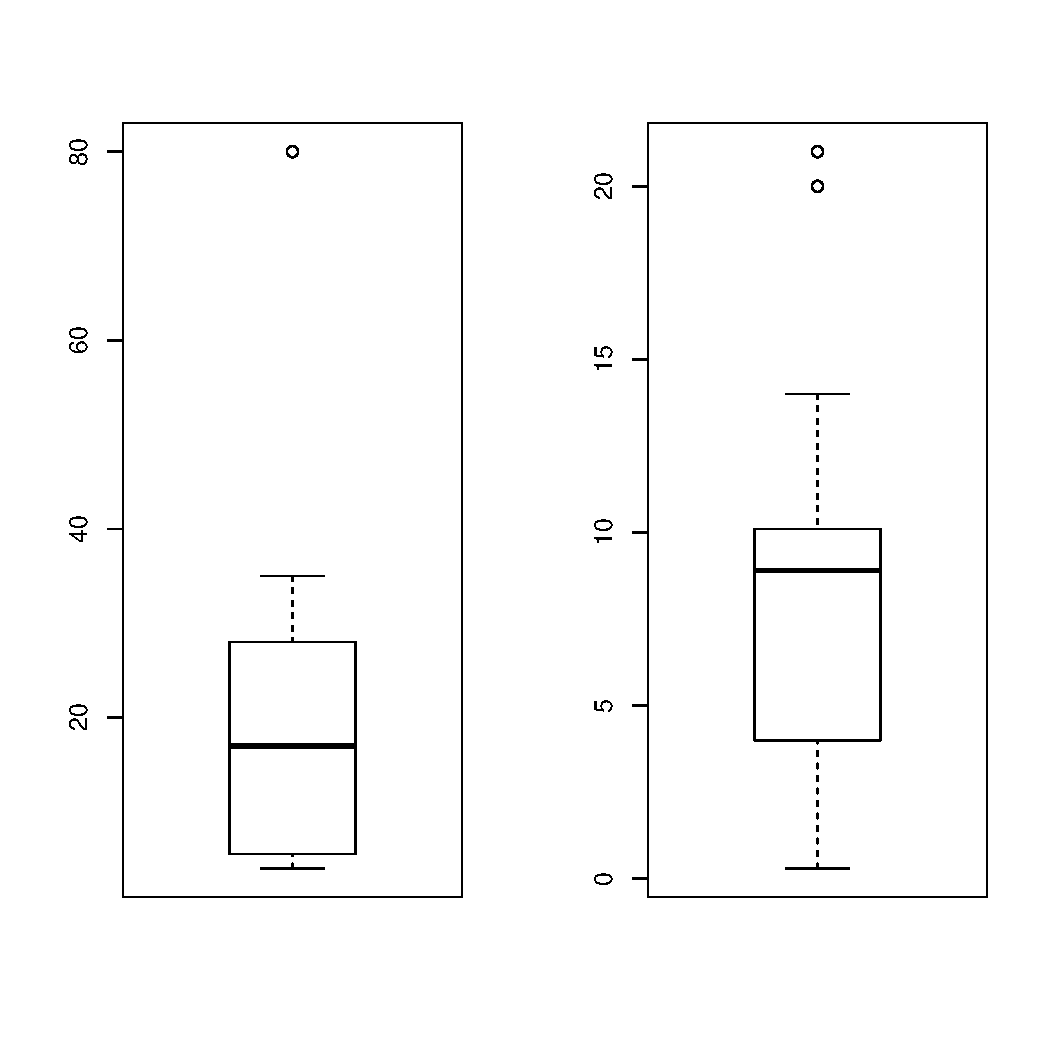
\includepdf[pages={1}]{img/Problem10.pdf}

%%% DONE
\section*{Problem 11}
\addcontentsline{toc}{section}{Eleventh Problem}

	Find the expected value and variance of the exponential distribution with parameter $\lambda$. 
	Show work.
	
	\paragraph{Answer}
	Find E[X] and V[X]. with $f(x) = \lambda e^{-\lambda x}$.
	\begin{displaymath}
		E[X] = \int_{0}^{\infty} x\lambda e^{-\lambda x} dx
	\end{displaymath}
	Begin by doing integration by parts:
	\begin{tabular}{ c c }
		$u = x$ & $dv= \lambda e^{-\lambda x}$ \\
		$du=dx$ & $v=\frac{\lambda e^{-\lambda x}}{-\lambda}$
	\end{tabular}
	\begin{displaymath}
		= x(-e^{-\lambda x})|_{0}^{\infty} - \int_{0}^{\infty} -e^{\lambda x} dx
	\end{displaymath}
	\begin{displaymath}
		= xe^{-\lambda x}|_{0}^{\infty} + \frac{e^{-\lambda x}}{-\lambda}|_{0}^{\infty}
	\end{displaymath}
	\centerline{$xe^{-\lambda x}|_{0}^{\infty} = (lim_{b\to\infty}-be^{-\lambda x}) - 0$ and $\frac{e^-\lambda x}{-\lambda}|_{0}^{\infty} = \frac{-1}{\lambda}\left[\lim_{b\to\infty}e^{-\lambda x} - 1\right] = \frac{-1}{\lambda}(-1)$}
	\begin{displaymath}
		Therefore: E[X] = \frac{1}{\lambda}
	\end{displaymath}
	
	Now we want to find $V[X] = E[X^2] - (E[X])^2$.
	\begin{displaymath}
		E[X^2] = \int_{0}^{\infty}x^2 f(x)dx
	\end{displaymath}
	\begin{displaymath}
		E[X^2] = \int_{0}^{\infty}x^2 \lambda e^{-\lambda x}dx
	\end{displaymath}
	Once again, do integration by parts:
	\begin{tabular}{ c c }
		$u = x^2$ & $dv= \lambda e^{-\lambda x}$ \\
		$du=2x$ & $v=\frac{\lambda e^{-\lambda x}}{-\lambda}$
	\end{tabular}
	\begin{displaymath}
		= \lambda\left[\frac{-1}{\lambda}x^2e^{-\lambda x}-\int2x\frac{e^{-\lambda x}}{-\lambda} dx
		\right]
	\end{displaymath}
	\begin{displaymath}
		= \lambda\left[\frac{1}{\lambda}\left[-x^2e^{-\lambda x}+2\int xe^{-\lambda x} dx\right]\right]
	\end{displaymath}
	\begin{displaymath}
		= -x^2e^{-\lambda x}+2\left[\frac{-1}{\lambda}xe^{-\lambda x}-\int\frac{e^{-\lambda x}}{-
		\lambda}dx\right]
	\end{displaymath}
	\begin{displaymath}
		= -x^2e^{-\lambda x}+2\left[\frac{-1}{\lambda}xe^{-\lambda x}+\frac{1}{\lambda}\int e^{-
		\lambda x}dx\right]
	\end{displaymath}
	\begin{displaymath}
		= -x^2e^{-\lambda x} + \frac{2}{\lambda}\left[-xe^{-\lambda x} + \frac{e^{-\lambda x}}{-
		\lambda}\right]
	\end{displaymath}
	\begin{displaymath}
		-e^{-\lambda x}\left(x^2+\frac{2}{\lambda}(x+\frac{1}{\lambda})\right)|_{0}^{\infty}
	\end{displaymath}
	\begin{displaymath}
		= 0 + 1\left(\frac{2}{\lambda} * \frac{1}{\lambda}\right)
	\end{displaymath}
	\begin{displaymath}
		E[X^2] = \frac{2}{\lambda^2}
	\end{displaymath}
	 FINALLY
	 \begin{displaymath}
	 	V[X] = E[X^2] - \left(E[X]\right)^2
	\end{displaymath}
	\begin{displaymath}
		V[X] = \frac{2}{\lambda^2} - \left(\frac{1}{\lambda}\right)^2 = \frac{2}{\lambda^2} - \frac{1}
		{\lambda^2}
	\end{displaymath}
	\begin{displaymath}
		V[X] = \frac{1}{\lambda^2}
	\end{displaymath}
	

\iffalse % We don't have to do this problem because we didn't cover how to do it in class.
\section*{Problem 12} 
\addcontentsline{toc}{section}{Twelfth Problem}

	Problem 2.45 on page 95 of the text (this should be done after class on 4/14).
	% Write out problem here

	\paragraph{Answer}
\fi
\vspace{20em} %%% DONE
\section*{Lab 2 Printouts}
\addcontentsline{toc}{section}{Lab 2 Printouts}

	Lab 2 printouts are attached.

% Inlcude PDF graph printouts for Lab 2
\clearpage
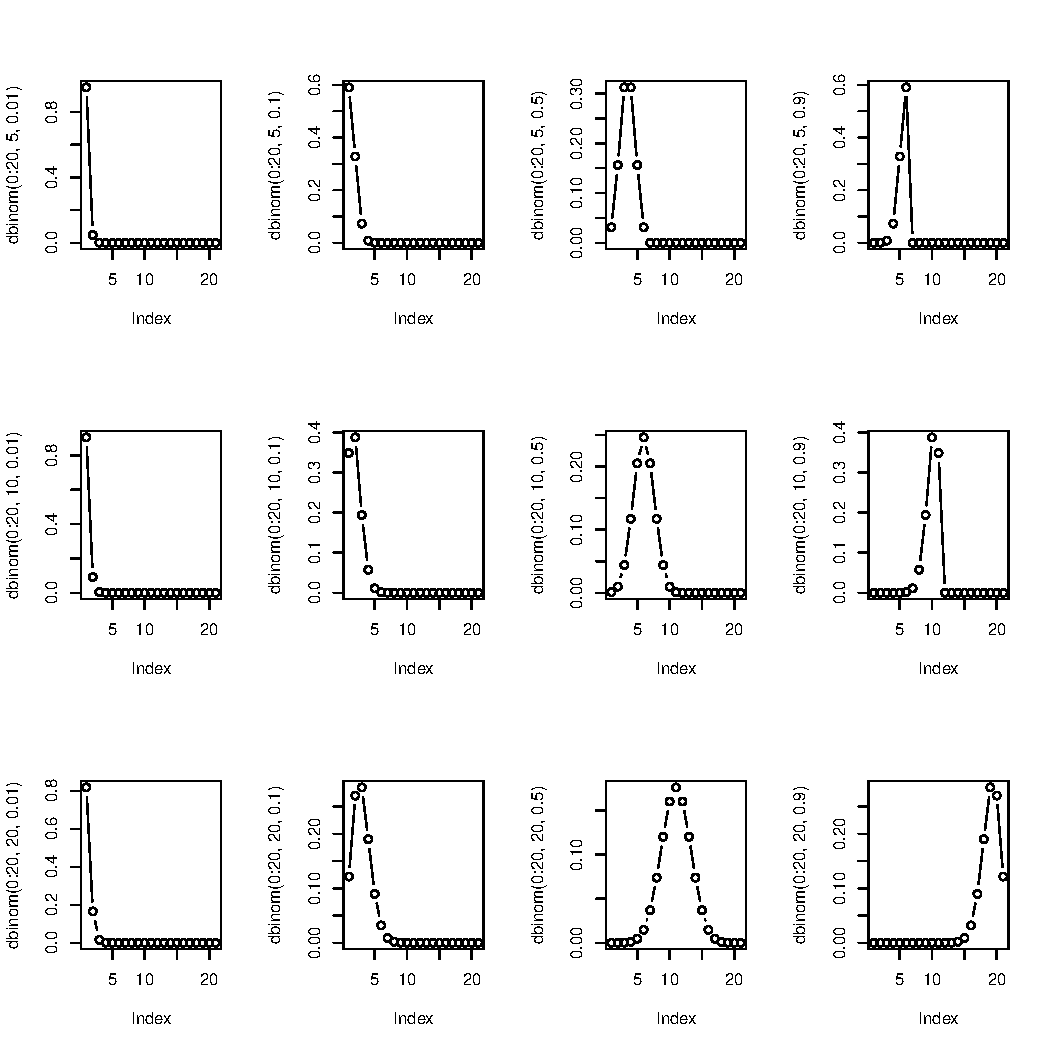
\includepdf[pages={1}]{img/Lab2FirstGraphs.pdf}
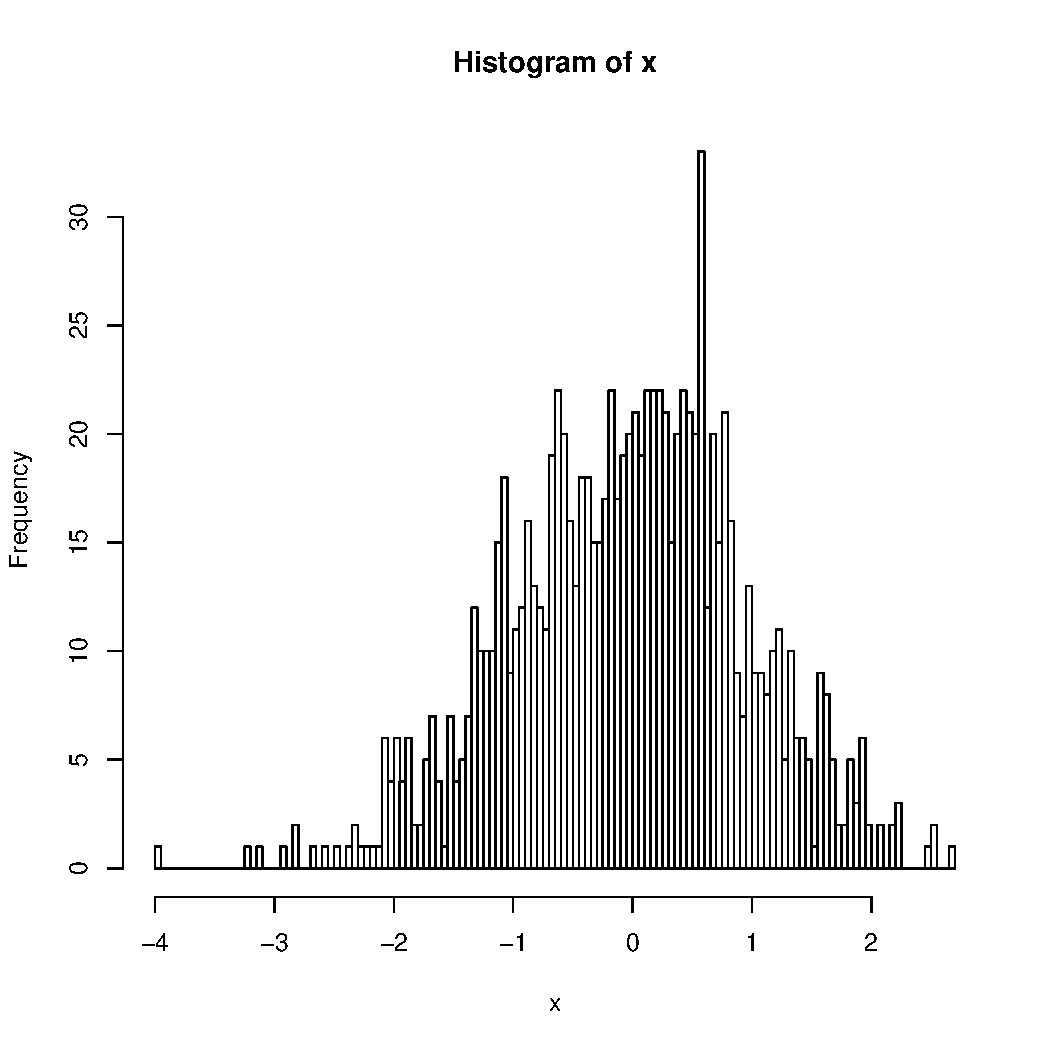
\includepdf[pages={1}]{img/NormalSample.pdf}
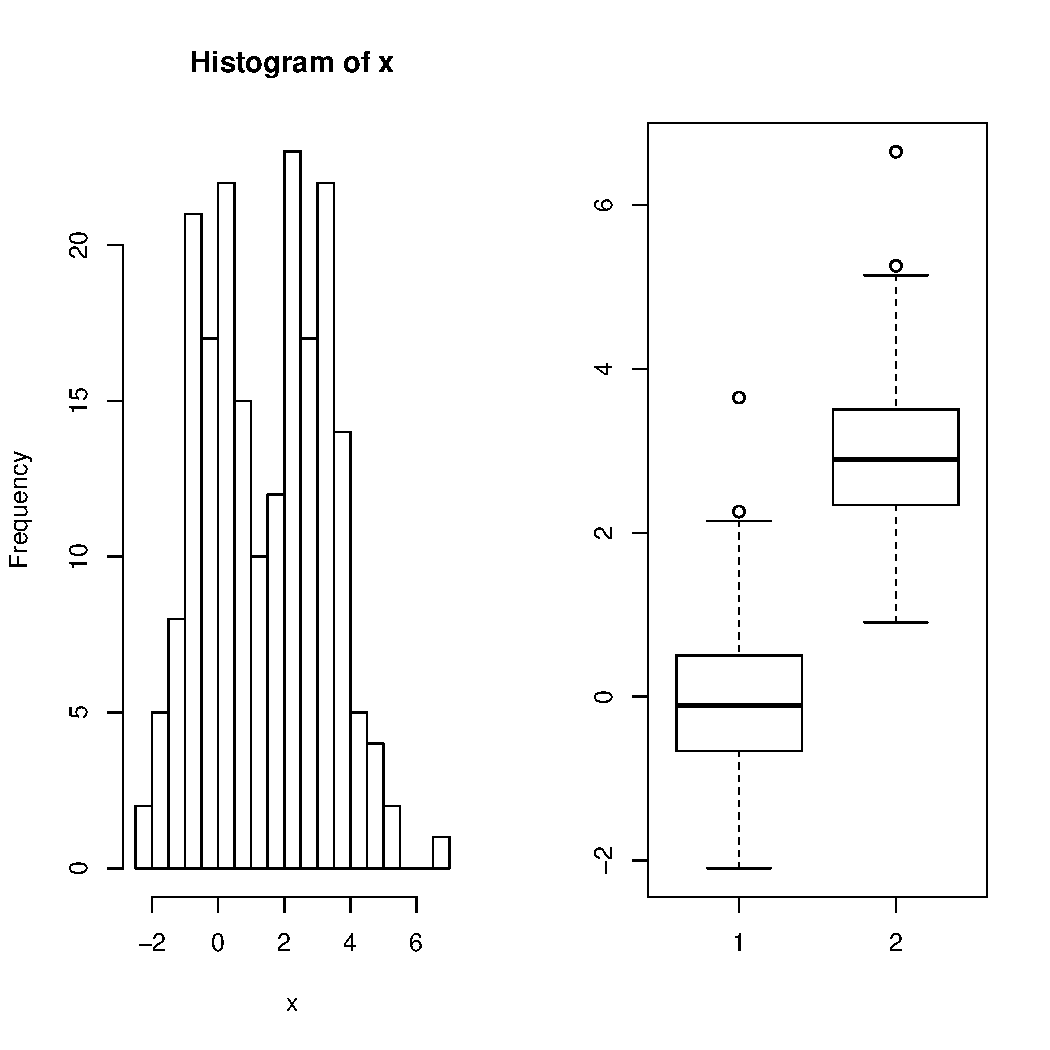
\includepdf[pages={1}]{img/boxplots.pdf}
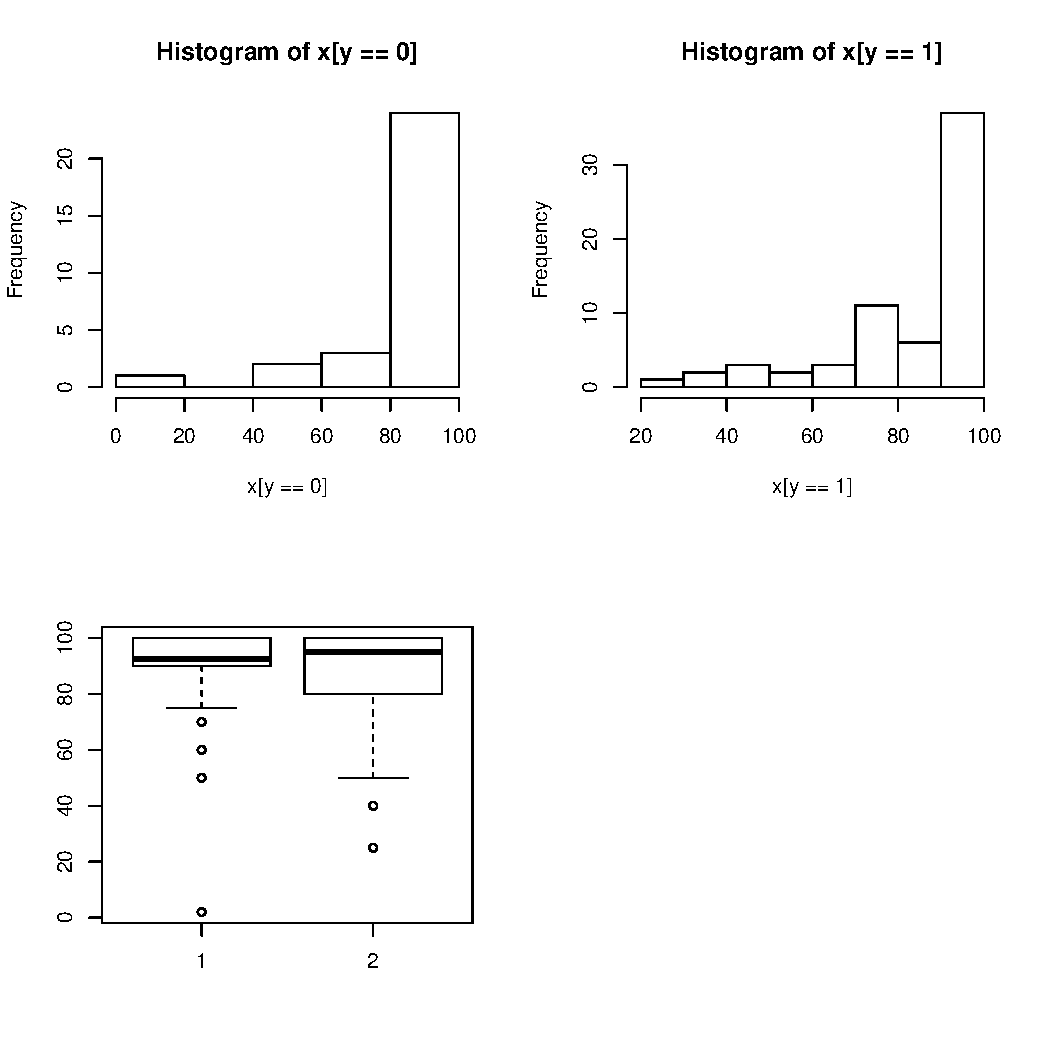
\includepdf[pages={1}]{img/AttendanceData.pdf}
	
\end{document}